\appendix
\section{Derivation of the variance comparisons}
Write $Y=m(S)+\varepsilon$, with $\mathbb E[\varepsilon\mid S]=0$. Orthogonality gives
\begin{align*}
 nV(h)&=\mathbb E[\operatorname{Var}(Y\mid S)]
       +\operatorname{Var}(m-h)+r\operatorname{Var}(h)\\
 &=\operatorname{Var}(Y)-2\operatorname{Cov}(m,h)
       +(1+r)\operatorname{Var}(h).
\end{align*}
Completing the square proves~\eqref{eq:identity}. Restricting $h$ to a fixed linear span replaces centered $m$ by its orthogonal projection into that span. Pythagoras then proves~\eqref{eq:projection}. The scalar case follows by differentiating the quadratic in $a$. When $m$ is affine, centered $m$ already belongs to the scalar span. When $m$ is constant, every nonconstant control adds variance to the label-only estimator.

For the fitted-control result, assume a fixed number $K=2$ of folds with positive limiting size fractions, fixed basis dimension, finite second moments of $Y$ and $B(S)$, nonsingular population basis covariance, consistent fitted coefficients, $n/N\to r\in(0,\infty)$, and positive limiting oracle variance. Let $\gamma$ be the population centered-regression coefficient, $b^*=\gamma/(1+n/N)$, $w_k=n_k/n$, and $\widehat b_{-k}$ the coefficient fit outside fold $k$. The exact remainder relative to the deterministic-control estimator is
\[
 \widehat\mu_{\rm cf}-\widehat\mu_{B^\top b^*}
 =\sum_{k=1}^2 w_k(\overline B_U-\overline B_{L_k})^\top
             (\widehat b_{-k}-b^*).
\]
Each feature-mean difference is $O_p(n^{-1/2}+N^{-1/2})$ and each coefficient error is $o_p(1)$; therefore the finite sum is $o_p(n^{-1/2})$. Shared unlabeled observations across folds do not invalidate this product-order argument. Coefficient error itself need not be smaller than a sample-mean fluctuation. Consistency of coefficients and sample second moments makes the out-of-fold residual variance and averaged-control unlabeled variance converge to the oracle components. The independent-sample central limit theorem and Slutsky's theorem then give $(\widehat\mu_{\rm cf}-\mu)/\widehat{\rm SE}\Rightarrow\mathcal N(0,1)$. This is an asymptotic result with stable dimension and consistent fitting; it supplies no finite-$n$ guarantee for rare events or poorly conditioned fits.

\section{Finite-sample coverage proof}
Condition on the training observations. The control is fixed and has its stated known range. The empirical Bernstein inequality applied in both directions to the evaluation residual mean fails with probability at most $\alpha/2$; the same holds for the independent unlabeled control mean. On their simultaneous event, their sum differs from $\mu$ by at most~\eqref{eq:finite}. The union bound gives conditional coverage at least $1-\alpha$; taking expectation over training preserves it. Since $\mu\in[0,1]$, intersecting the resulting interval with that known parameter space cannot remove the true mean. Independence from evaluation labels and correct support bounds are essential assumptions.

\section{Experimental and reproduction details}\label{app:reproduction}
\paragraph{Synthetic populations.}
Independently draw all labeled and unlabeled scores uniformly on $[0,1]$. Write $T=2S-1$; all noise terms below are independent of scores and of each other. The linear population has $Y=.2+.8S+\epsilon$, $\epsilon\sim\mathcal N(0,.2^2)$, with mean $.6$. The quadratic population has $Y=T^2+\epsilon$, $\epsilon\sim\mathcal N(0,.15^2)$, with mean $1/3$. The sigmoid population has $Y=(1+\exp(-12(S-.5)))^{-1}+\epsilon$ with the same $.15$ Gaussian noise and mean $.5$. The no-signal population has $Y=.4+\epsilon$, $\epsilon\sim\mathcal N(0,.2^2)$, with mean $.4$. Heavy-tailed quadratic data use $Y=T^2+.15t_3$, with mean $1/3$ and finite noise variance $3(.15)^2$. Quadratic Bernoulli data use $Y\mid S\sim\operatorname{Bernoulli}(.05+.9T^2)$ with mean $.35$. Rare binary data use $Y\sim\operatorname{Bernoulli}(.01)$ independently of $S$. The bounded supplement has $Y=.025+.95T^2+\epsilon$, $\epsilon\sim\operatorname{Uniform}[-.025,.025]$, with mean $.025+.95/3$ and known support $[0,1]$.

The bounded supplement was specified before inspecting the main results to test range penalties in a designed high-signal regime. The equal-$n,N$ supplement followed inspection of initial real/bounded findings; it is a follow-up, not a preregistered original-grid experiment. No method or basis degree was selected by evaluation labels. The exact projection calculations, including their parameters, are generated by \path{code/theory.py}. The quadratic oracle/scalar ratio is
\[
\sqrt{\frac{.15^2+(4/45)r/(1+r)}{.15^2+4/45}},\qquad r=n/N.
\]
The analytical values and their interpretation are presented separately from measured performance.

\paragraph{Empirical populations and data provenance.}
The PPI v0.2.3 example archives contain 16,743 galaxy records, 1,596 forest records and 10,802 AlphaFold records. Each provides binary archived labels and scores in $[0,1]$. The empirical mean labels are $.2592725318$, $.1516290727$, and $.1773745603$, respectively. The labels are reference annotations for this benchmark, not asserted error-free physical truth. The original study descriptions and examples are in \citet{angelopoulos2023ppi}; we use neither all of Galaxy Zoo 2 nor a new scientific sampling frame. The archive's unlabeled sample is simulated by hiding outcomes of independent with-replacement draws, not by relabeling or expanding the labeled draw.

\path{provenance/manifest.json} gives pinned source URLs, byte sizes, SHA-256 values and versions. \path{code/download_data.py} checks existing files or retrieves the three exact package-declared Drive IDs. The reference package's code is MIT licensed; a separate license for its NPZ data is not established by the supplied documentation. We do not infer that the code's license covers the data; original data terms require checking before external redistribution. The official venue files retain their original provenance, and no separate template license is inferred.

\paragraph{Baseline implementation and fitting.}
The default scalar baseline reproduces \texttt{ppi-python==0.2.3}: covariance uses divisor $n$, pooled score variance uses divisor $n+N-1$, the tuning denominator includes $1+n/N$, and automatic tuning clips to $[0,1]$. The unrestricted scalar removes only clipping. Normal standard-error components use divisor $n$ or $N$, matching the reference. Twenty-four interval comparisons against the installed package agree with maximum endpoint difference $1.11\times10^{-16}$ (\path{results/verification.json}). A Legendre coordinate $P_1(2S-1)=2S-1$ therefore receives half the coefficient expressed on $S$; constants cancel.

The cubic uses $P_1,P_2,P_3$, centered least squares, two equal deterministic folds, and shrinkage $1/(1+n/N)$. Least squares uses a Moore--Penrose solution with relative singular-value cutoff $10^{-10}$. Intercepts cancel in the Wald correction. The degree-12 variants and same-label cubic are fixed diagnostics; there is no regularization or degree search. Numerically truncated or poorly conditioned fits can fail the coefficient-consistency condition; the asymptotic argument does not override that requirement. For EB, training uses $q=\max(10,\lfloor n/4\rfloor)$ labels, requiring $n-q\ge2$ and $N\ge2$. The scalar coefficient is clipped to $[0,1]$ before shrinkage; the cubic includes an intercept, clips predictions to $[0,1]$ and then shrinks by $1/(1+(n-q)/N)$. These known ranges supply the guarantee. Label-only and all-label unit-control EB need no training split. All Wald intervals remain untruncated, including degenerate and extreme outcomes; EB and exact binary intervals use the known parameter range.

\paragraph{Seeds and uncertainty.}
The root seed is 20261102. A draw uses NumPy \texttt{SeedSequence([seed, scenario\_ordinal, n, N/n, rep])}, where the fixed scenario order is linear, quadratic, sigmoid, no signal, heavy tail, quadratic Bernoulli, rare binary, galaxies, forest, AlphaFold, bounded quadratic. Repetition IDs start at zero. The internal output name \texttt{null} was renamed \texttt{no\_signal} because standard CSV readers interpreted the former as missing data; its ordinal and measurements are unchanged. No incomplete or failed trial is removed from reported summaries.

For paired widths $A_i,B_i$ and $R$ repetitions, $\widehat\rho=\bar A/\bar B$ has Monte Carlo standard error
\[
 \widehat{\operatorname{SE}}(\widehat\rho)
 =\frac{\operatorname{sd}(A_i-\widehat\rho B_i)}{\sqrt R\,\bar B}.
\]
Reported ratio intervals use $\widehat\rho\pm1.96\widehat{\operatorname{SE}}$. Width-mean standard errors use the across-repetition sample standard deviation divided by $\sqrt R$. These quantify Monte Carlo estimation uncertainty, not a target-parameter confidence interval or a width-distribution percentile band. Coverage intervals are two-sided Wilson intervals for the integer hit counts. At coverage near $.95$, 5,000 repetitions give approximately $.006$ half-width, so smaller coverage differences cannot be resolved sharply. Exploratory exact-binomial tests and Holm adjustments are retained in \path{results/coverage_diagnostics.csv}.

\paragraph{Environment, commands and compute.}
The analyses used Python 3.11.2, NumPy 2.4.6, SciPy 1.17.1, pandas 3.0.6 and PyArrow 26.0.0. Figure-generation versions are in \path{presentation/render_manifest.json}; the manuscript uses TeX Live 2022, latexmk 4.79 and the unmodified official NeurIPS 2026 style. Run from the delivery root after installing \path{code/requirements.txt}, with \texttt{OPENBLAS\_NUM\_THREADS=1} and \texttt{OMP\_NUM\_THREADS=1}. Exact reproduction commands are in \path{analysis/README.md}; the main commands are \path{code/run_experiments.py} with the synthetic/real groups, 5,000 repetitions and $n=100,500,2000$, followed by exact/full-label EB baseline additions and \path{code/summarize.py}. Include all four result directories, including \texttt{ratio1}, when regenerating summaries and audits. The figure/table mapping and command are in \path{presentation/README.md} and \path{presentation/captions.md}. Build the paper with \texttt{bash manuscript/build.sh}; numerical prose is imported from the supplied summaries by \path{manuscript/import_numbers.py}, which records input hashes.

CPU-only jobs ran with the sandbox's two-CPU and 4096\,MB memory ceilings on a shared host, without a GPU or paid API. Recorded elapsed times are \SyntheticSeconds{}\,s for the main synthetic grid, \RealSeconds{}\,s for real data, \BoundedRunSeconds{}\,s for bounded data, and \RatioRunSeconds{}\,s for the equal-$n,N$ follow-up. Their sum is run elapsed time, not measured CPU consumption or total project time; shared-host load affects reruns. An approximate rerun budget is tens of minutes for the experiments and postprocessing, excluding downloads and environment setup. This is an estimate. Timing pilots and postprocessing are recorded separately in \path{analysis/run_log.md}.

All main experiments completed. Initial reference-package import failed because dependencies were missing, then succeeded after installation. A first finalization job was intentionally stopped after 20.668\,s to replace slow repeated row assignments; completed baseline additions were retained idempotently. This was a postprocessing change, not exclusion or rerunning of unfavorable experiments. Extreme widths and undercoverage remain in all summaries; degree-12 diagnostics were not promoted to the primary method. No main experiment is represented by a pilot.

\paragraph{Source boundaries and LLM disclosure.}
Only the supplied starter papers, exact version-pinned reference package paths, the directly addressed unrelated empirical-Bernstein reference, and official format/ethics pages were consulted. Broad literature and citation-chain searches were avoided under the task's independence restriction. No prohibited source was sought or identified as encountered. The bounded source review cannot establish exhaustive priority or novelty; \path{manuscript/source-consultation.md} records the manuscript's sources. LLM-based research agents participated in study design, mathematical exposition, implementation, review and manuscript preparation. Reported empirical evidence comes from executed numerical code; no LLM-generated outcome labels or model predictions were used as experimental evidence.

\section{Analytical oracle limits}\label{app:oracle}
\begin{table}[ht]
\caption{Analytical leading-order width ratios within the score-control class. The oracle uses $h^*=\mathbb E[Y\mid S]/(1+n/N)$; the scalar uses its population-optimal unrestricted coefficient. Entries are square roots of exact variances from \texttt{code/theory.py}, rendered by \texttt{presentation/render.py}. They are theoretical predictions, not measured widths or finite-sample coverage guarantees.}
\centering% Generated by presentation/render.py; do not edit numeric values.
\begin{tabular}{lrrr}
\toprule
Regime & $n/N$ & Oracle / scalar & Oracle / label \\
\midrule
Linear & 0.1 & 1.000 & 0.693 \\
Linear & 1 & 1.000 & 0.845 \\
Quadratic & 0.1 & 0.524 & 0.524 \\
Quadratic & 1 & 0.775 & 0.775 \\
No signal & 0.1 & 1.000 & 1.000 \\
No signal & 1 & 1.000 & 1.000 \\
Heavy-tailed noise & 0.1 & 0.695 & 0.695 \\
Heavy-tailed noise & 1 & 0.846 & 0.846 \\
Quadratic Bernoulli & 0.1 & 0.844 & 0.844 \\
Quadratic Bernoulli & 1 & 0.917 & 0.917 \\
Bounded quadratic & 0.1 & 0.305 & 0.305 \\
Bounded quadratic & 1 & 0.708 & 0.708 \\
\bottomrule
\end{tabular}

\end{table}


\clearpage
\section{Complete evidence displays}\label{app:displays}
All figures below target $\mu=\mathbb E[Y]$ with nominal 95\% intervals. Coverage bars are 95\% Wilson Monte Carlo intervals; width-ratio bars are paired delta-method 95\% Monte Carlo intervals, not target-parameter intervals. Ratios divide paired mean widths, and values below one indicate narrowing. Every trial remains in the summaries. All figures and tables are generated by \path{presentation/render.py}; \path{presentation/captions.md} maps each output to its exact inputs and generator function, and \path{presentation/render_manifest.json} records their hashes.

\begin{table}[ht]
\caption{Large-label main-grid comparisons at $n=2000,N=20000,R=5000$. Coverage includes 95\% Wilson Monte Carlo intervals. Width ratio is cubic/PPI++ mean width, $\pm1.96$ paired Monte Carlo standard errors. Archive rows target empirical populations. Narrowing with undercoverage is not a valid improvement; compatibility with nominal coverage is not a proof. Absolute widths are retained in Appendix~\ref{app:complete}.}
\centering% Generated by presentation/render.py; do not edit numeric values.
\begin{tabular}{lrrr}
\toprule
Regime & PPI++ coverage & Cubic coverage & Width ratio \\
\midrule
Linear & 0.948 [0.941, 0.954] & 0.948 [0.942, 0.954] & 1.00119 $\pm$ 0.00004 \\
Quadratic & 0.949 [0.942, 0.954] & 0.950 [0.944, 0.956] & 0.52480 $\pm$ 0.00020 \\
Sigmoid & 0.945 [0.939, 0.951] & 0.949 [0.942, 0.954] & 0.85365 $\pm$ 0.00019 \\
No signal & 0.952 [0.946, 0.958] & 0.952 [0.946, 0.958] & 1.00145 $\pm$ 0.00005 \\
Heavy-tailed noise & 0.946 [0.939, 0.952] & 0.950 [0.944, 0.956] & 0.69245 $\pm$ 0.00098 \\
Quadratic Bernoulli & 0.948 [0.941, 0.953] & 0.949 [0.943, 0.955] & 0.84537 $\pm$ 0.00029 \\
Rare Bernoulli & 0.949 [0.942, 0.955] & 0.943 [0.937, 0.949] & 1.00140 $\pm$ 0.00005 \\
Galaxies & 0.949 [0.943, 0.955] & 0.949 [0.942, 0.955] & 1.00141 $\pm$ 0.00007 \\
Forest & 0.949 [0.943, 0.955] & 0.947 [0.941, 0.953] & 0.99894 $\pm$ 0.00014 \\
AlphaFold & 0.944 [0.937, 0.950] & 0.949 [0.943, 0.955] & 1.00150 $\pm$ 0.00015 \\
\bottomrule
\end{tabular}

\label{tab:main}
\end{table}

\begin{table}[ht]
\caption{Coverage scope and additional conditions for implemented families. Independent iid draws from a common population underpin score-control comparisons; CP uses iid binary labels. Cross-fitting alone gives no finite-sample guarantee. EB uses known support ranges and the stated concentration allocation; trained controls must be independent of evaluation labels conditional on training.}
\centering% Generated by presentation/render.py; do not edit numeric values.
\begin{tabular}{@{}p{1.25in}p{2.9in}p{1.0in}@{}}
\toprule
Family & Additional conditions & Coverage scope \\
\midrule
Label/PPI/scalar Wald & Controls h=0, S, or aS; finite second moments; consistent variance and applicable normal limit. & Asymptotic \\
Cross-fit fixed basis & Prespecified Legendre basis; fixed dimension; nonsingular covariance; consistent coefficients/variance; finite second moments. & Asymptotic \\
Bounded EB label/PPI & $Y,S\in[0,1]$; known control range; independent common-population iid draws; stated error allocation. & Finite sample \\
Trained scalar/cubic EB & As above, with training independent of evaluation labels and bounded clipped control. & Finite sample \\
Clopper--Pearson & Binary iid labels from the target population. Uses no predictor. & Finite sample \\
\bottomrule
\end{tabular}

\label{tab:assumptions}
\end{table}

\clearpage
\begin{figure}[p]
\centering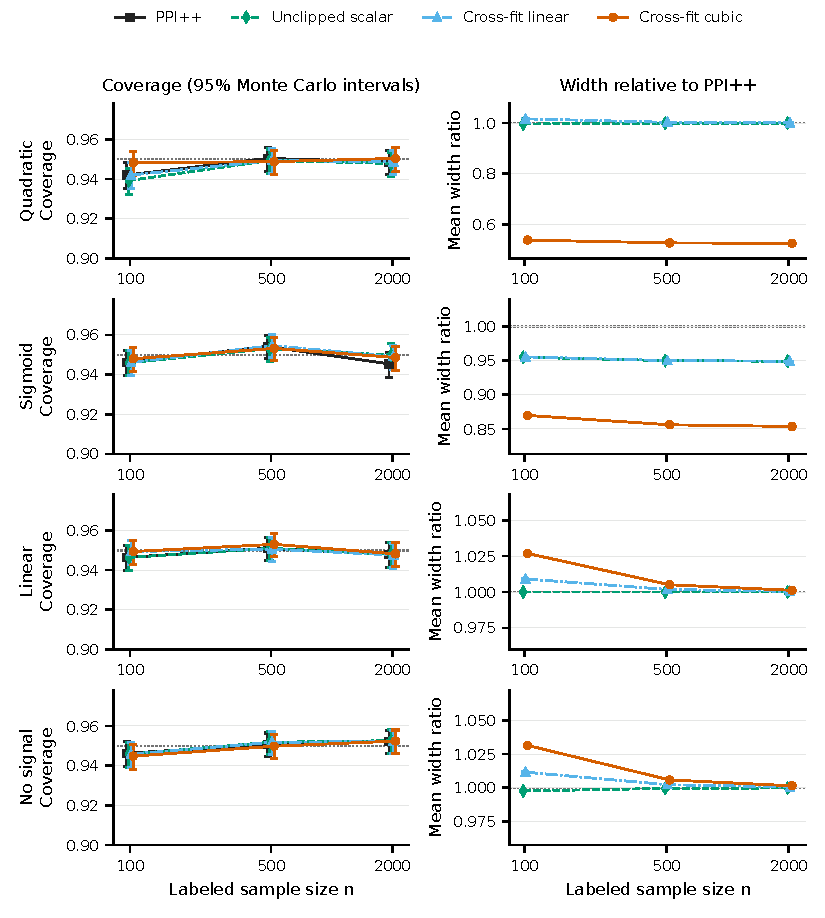
\includegraphics[width=\linewidth]{figures/synthetic.pdf}
\caption{Dependence on label count in quadratic, sigmoid, affine and no-signal populations, with $N=10n,R=5000$ per setting. Coverage and paired mean-width ratios to PPI++ use the Monte Carlo intervals defined above. Unrestricted scalar and cross-fit linear controls distinguish nonlinear information from scalar clipping and fitting cost. Axes vary by row to retain all uncertainty endpoints and expose small costs alongside large gains; horizontal offsets separate overlapping methods. These are asymptotically justified Wald intervals.}
\label{fig:synthetic}
\end{figure}
\clearpage
\begin{figure}[p]
\centering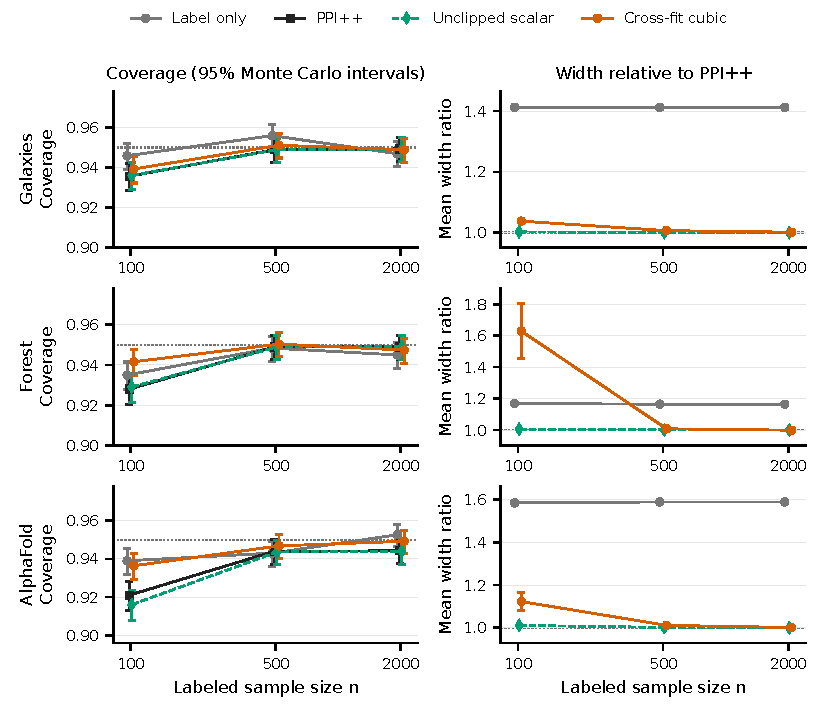
\includegraphics[width=\linewidth]{figures/real.pdf}
\caption{Archived-score results show small-label fitting costs and negligible large-label nonlinear gain. Independent with-replacement draws target each archive's empirical mean, with no broader population claim; $N=10n,R=5000$ per setting. Coverage uses Wilson 95\% Monte Carlo intervals; mean-width ratios to PPI++ use paired delta-method 95\% Monte Carlo intervals. Width means retain unstable large fits. These Wald intervals have asymptotic justification.}
\label{fig:real}
\end{figure}
\clearpage
\begin{figure}[p]
\centering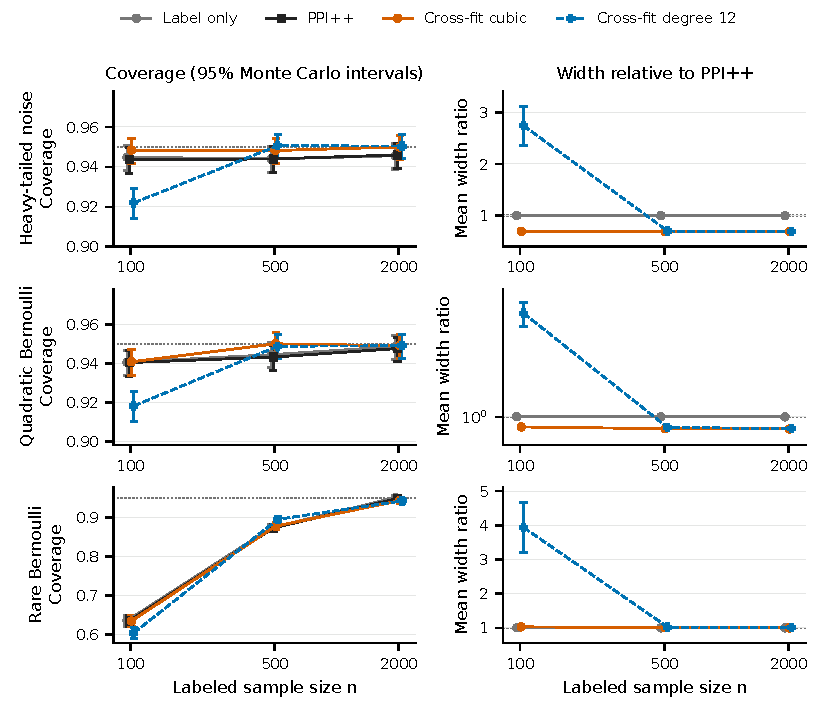
\includegraphics[width=\linewidth]{figures/stress.pdf}
\caption{Heavy tails, nonlinear binary outcomes, rare events and a fixed degree-12 cross-fit diagnostic expose finite-sample limitations; $N=10n,R=5000$. Coverage uses Wilson 95\% Monte Carlo intervals, and mean-width ratios to PPI++ use paired delta-method 95\% Monte Carlo intervals. Cross-fitting does not ensure finite-sample validity or stable fitting, and short rare-event Wald intervals fail. The quadratic-Bernoulli width panel is logarithmic; other panels are linear. Axis ranges retain all uncertainty endpoints. Every trial remains in the means.}
\label{fig:stress}
\end{figure}
\clearpage
\begin{figure}[p]
\centering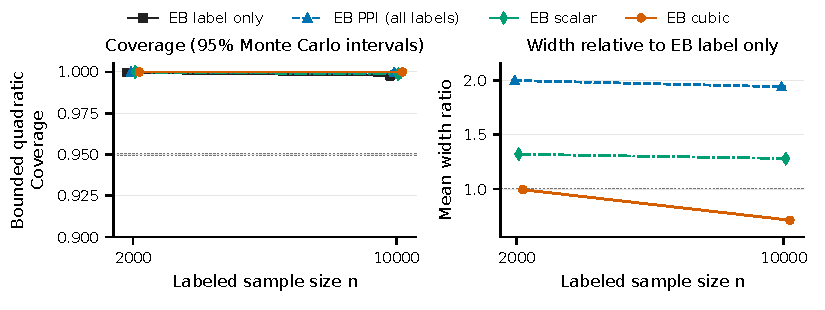
\includegraphics[width=\linewidth]{figures/finite.pdf}
\caption{Sample-size dependence of the bounded high-signal quadratic EB comparison; $N=10n,R=3000$. All training consumes the original $n$ labels. Coverage uses Wilson 95\% Monte Carlo intervals, and mean-width ratios to EB label-only use paired delta-method 95\% Monte Carlo intervals. At $n=2000$ range penalties nearly erase the gain; at $n=10000$ cubic EB is shorter while conservative. The $\ge95\%$ guarantee follows from known-range concentration and independent training, independently of these hit counts.}
\label{fig:boundedn}
\end{figure}
\clearpage
\begin{figure}[p]
\centering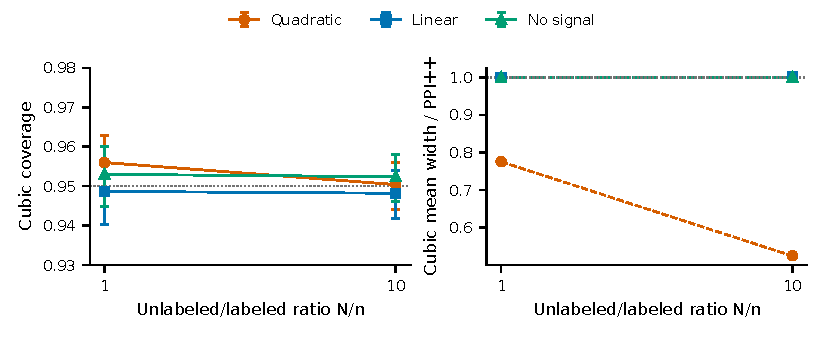
\includegraphics[width=\linewidth]{figures/finite_n.pdf}
\caption{Finite unlabeled information limits the gain. At $n=2000$, $N/n=1$ uses $R=3000$ (a declared follow-up) and $N/n=10$ uses $R=5000$ (main grid). Left: cubic coverage with Wilson 95\% Monte Carlo intervals. Right: paired cubic/PPI++ mean-width ratios with delta-method 95\% Monte Carlo intervals. Dashed lines are analytical oracle/unrestricted-scalar ratios, not empirical fits. Linear/no-signal oracle curves coincide at one. This is a class-restricted asymptotic comparison, not a universal interval-length bound. Methods share identical inputs within each setting.}
\label{fig:finiteN}
\end{figure}

\clearpage
\section{Finite-sample comparisons and fitting diagnostics}
\begin{table}[ht]
\caption{Bounded-quadratic finite-sample comparison, $N=10n,R=3000$. Coverage has Wilson 95\% Monte Carlo intervals. Width is the absolute mean in outcome units, with its Monte Carlo standard error in parentheses. Ratios to EB label-only report $\pm1.96$ paired Monte Carlo standard errors. Training uses the original budget; label-only and fixed-PPI use all $n$. Guarantees follow from assumptions, not observed coverage.}
\centering% Generated by presentation/render.py; do not edit numeric values.
\begin{tabular}{rlrrr}
\toprule
$n$ & Method & Coverage & Mean (MCSE) & Width / EB label \\
\midrule
2000 & EB label only & 1.000 [0.998, 1.000] & 0.04779 ($8.4\times 10^{-6}$) & 1 (reference) \\
2000 & EB PPI (full) & 1.000 [0.999, 1.000] & 0.09555 ($1.8\times 10^{-5}$) & 1.99949 $\pm$ 0.00070 \\
2000 & EB scalar & 1.000 [0.999, 1.000] & 0.06311 ($2.1\times 10^{-5}$) & 1.32075 $\pm$ 0.00076 \\
2000 & EB cubic & 1.000 [0.999, 1.000] & 0.0475 ($1.7\times 10^{-6}$) & 0.99400 $\pm$ 0.00032 \\
10000 & EB label only & 0.998 [0.996, 0.999] & 0.01884 ($1.6\times 10^{-6}$) & 1 (reference) \\
10000 & EB PPI (full) & 1.000 [0.998, 1.000] & 0.03657 ($3.6\times 10^{-6}$) & 1.94153 $\pm$ 0.00035 \\
10000 & EB scalar & 0.999 [0.997, 0.999] & 0.02411 ($3.3\times 10^{-6}$) & 1.28012 $\pm$ 0.00027 \\
10000 & EB cubic & 1.000 [0.999, 1.000] & 0.01343 ($3.4\times 10^{-7}$) & 0.71279 $\pm$ 0.00011 \\
\bottomrule
\end{tabular}

\label{tab:finite}
\end{table}
\begin{table}[ht]
\caption{Exact binary CP and bounded EB comparisons, $N=10n,R=5000$. Five binary regimes at $n=2000$ and rare events at $n=100$ are retained. Coverage has Wilson 95\% Monte Carlo intervals; absolute mean widths have Monte Carlo standard errors in parentheses. CP is exact for binary iid labels. Archive rows target empirical populations under independent with-replacement draws. Fitted EB gives no archive-data gain.}
\centering% Generated by presentation/render.py; do not edit numeric values.
\begin{tabular}{lrlrr}
\toprule
Regime & $n$ & Method & Coverage & Mean (MCSE) \\
\midrule
Quadratic Bernoulli & 2000 & CP & 0.952 [0.946, 0.958] & 0.04228 ($4.2\times 10^{-6}$) \\
Quadratic Bernoulli & 2000 & EB label only & 0.999 [0.998, 1.000] & 0.07338 ($6.4\times 10^{-6}$) \\
Quadratic Bernoulli & 2000 & EB PPI (full) & 1.000 [0.999, 1.000] & 0.1173 ($1.5\times 10^{-5}$) \\
Quadratic Bernoulli & 2000 & EB scalar & 1.000 [0.999, 1.000] & 0.09531 ($2.3\times 10^{-5}$) \\
Quadratic Bernoulli & 2000 & EB cubic & 1.000 [0.999, 1.000] & 0.108 ($1.7\times 10^{-5}$) \\
Rare Bernoulli & 100 & CP & 0.984 [0.980, 0.987] & 0.0524 ($2.0\times 10^{-4}$) \\
Rare Bernoulli & 100 & EB label only & 1.000 [0.999, 1.000] & 0.1362 ($4.0\times 10^{-4}$) \\
Rare Bernoulli & 100 & EB PPI (full) & 1.000 [0.999, 1.000] & 0.3873 ($4.8\times 10^{-4}$) \\
Rare Bernoulli & 100 & EB scalar & 1.000 [0.999, 1.000] & 0.2 ($5.4\times 10^{-4}$) \\
Rare Bernoulli & 100 & EB cubic & 1.000 [0.999, 1.000] & 0.3605 ($5.2\times 10^{-4}$) \\
Rare Bernoulli & 2000 & CP & 0.960 [0.954, 0.965] & 0.009243 ($1.4\times 10^{-5}$) \\
Rare Bernoulli & 2000 & EB label only & 1.000 [0.999, 1.000] & 0.02158 ($3.8\times 10^{-5}$) \\
Rare Bernoulli & 2000 & EB PPI (full) & 1.000 [0.999, 1.000] & 0.05068 ($1.0\times 10^{-4}$) \\
Rare Bernoulli & 2000 & EB scalar & 1.000 [0.999, 1.000] & 0.02613 ($5.1\times 10^{-5}$) \\
Rare Bernoulli & 2000 & EB cubic & 1.000 [0.999, 1.000] & 0.03409 ($5.1\times 10^{-5}$) \\
Galaxies & 2000 & CP & 0.953 [0.947, 0.958] & 0.03888 ($6.7\times 10^{-6}$) \\
Galaxies & 2000 & EB label only & 1.000 [0.999, 1.000] & 0.06825 ($1.0\times 10^{-5}$) \\
Galaxies & 2000 & EB PPI (full) & 1.000 [0.999, 1.000] & 0.08179 ($1.5\times 10^{-5}$) \\
Galaxies & 2000 & EB scalar & 1.000 [0.999, 1.000] & 0.09331 ($2.2\times 10^{-5}$) \\
Galaxies & 2000 & EB cubic & 1.000 [0.999, 1.000] & 0.09395 ($2.0\times 10^{-5}$) \\
Forest & 2000 & CP & 0.950 [0.944, 0.956] & 0.03192 ($9.7\times 10^{-6}$) \\
Forest & 2000 & EB label only & 1.000 [0.999, 1.000] & 0.05772 ($1.5\times 10^{-5}$) \\
Forest & 2000 & EB PPI (full) & 1.000 [0.999, 1.000] & 0.07779 ($1.6\times 10^{-5}$) \\
Forest & 2000 & EB scalar & 1.000 [0.999, 1.000] & 0.08788 ($3.1\times 10^{-5}$) \\
Forest & 2000 & EB cubic & 1.000 [0.999, 1.000] & 0.0895 ($2.2\times 10^{-5}$) \\
AlphaFold & 2000 & CP & 0.956 [0.950, 0.961] & 0.03394 ($8.8\times 10^{-6}$) \\
AlphaFold & 2000 & EB label only & 0.999 [0.998, 1.000] & 0.06077 ($1.3\times 10^{-5}$) \\
AlphaFold & 2000 & EB PPI (full) & 1.000 [0.999, 1.000] & 0.06998 ($1.7\times 10^{-5}$) \\
AlphaFold & 2000 & EB scalar & 1.000 [0.999, 1.000] & 0.08089 ($2.2\times 10^{-5}$) \\
AlphaFold & 2000 & EB cubic & 1.000 [0.999, 1.000] & 0.08128 ($2.3\times 10^{-5}$) \\
\bottomrule
\end{tabular}

\label{tab:binary}
\end{table}
\clearpage
\begin{table}[ht]
\caption{Fitting diagnostics at $n=100,N=1000,R=5000$. Width medians, empirical 99th percentiles and maxima are computed from saved draws. CF denotes cross-fitting. Extreme fits remain in every mean and uncertainty estimate; high-degree cross-fitting is a diagnostic, not an automatically valid alternative. Absolute widths are in outcome units and need not share a scale across populations. Archive rows target empirical populations.}
\centering% Generated by presentation/render.py; do not edit numeric values.
\begin{tabular}{llrrr}
\toprule
Regime & Method & Median & 99th percentile & Maximum \\
\midrule
Quadratic & CF cubic & 0.069 & 0.080 & 0.088 \\
Quadratic & CF degree 12 & 0.090 & 2.717 & 33.471 \\
Quadratic & Plug-in degree 12 & 0.066 & 0.085 & 0.894 \\
No signal & CF cubic & 0.080 & 0.096 & 0.117 \\
No signal & CF degree 12 & 0.112 & 4.324 & 54.839 \\
No signal & Plug-in degree 12 & 0.074 & 0.097 & 0.562 \\
Galaxies & CF cubic & 0.125 & 0.159 & 0.216 \\
Galaxies & CF degree 12 & 0.183 & 232.088 & 258258.462 \\
Galaxies & Plug-in degree 12 & 0.112 & 0.141 & 0.538 \\
Forest & CF cubic & 0.132 & 1.607 & 35.827 \\
Forest & CF degree 12 & 17962.463 & 22647862.897 & 80256413.504 \\
Forest & Plug-in degree 12 & 0.128 & 11520.016 & 3277521.013 \\
AlphaFold & CF cubic & 0.101 & 0.152 & 8.749 \\
AlphaFold & CF degree 12 & 1.430 & 1544278.825 & 27793093.714 \\
AlphaFold & Plug-in degree 12 & 0.086 & 0.345 & 25.303 \\
\bottomrule
\end{tabular}

\label{tab:tails}
\end{table}
\clearpage
\section{Every completed method/setting cell}\label{app:complete}
The following tables retain all 405 cells, including all diagnostics and the equal-$n,N$ follow-up. Full paired comparisons are in \path{tables/all_paired.csv}; \path{tables/all_cells.csv} is the lossless summary export. Both are generated from the analysis summaries by \path{presentation/render.py}. EB split and full-label PPI are distinct. Archive cells use independent with-replacement sampling of the empirical population; all other cells use the stated synthetic laws.
\input{tables/full_results.tex}
\clearpage
